% =============================================================================
% CAPÍTULO 2 — a raiz: o que a soma guarda.
%
% O fracasso que o abre, com número na mão: somar as variações diárias do índice ao longo de
% \numSomaSerieDias{} pregões entrega \numSomaVariacoesPct\% onde o índice andou
% \numSomaVariacaoRealPct\% — a metade. Num mês as duas contas quase coincidem
% (\numSomaCurtaVariacoesPct\% contra \numSomaCurtaRealPct\%), e nada avisa que a diferença cresce
% com o horizonte.
%
% Medição: lab/experimentos/E22_soma.ipynb e E44_expoente.ipynb (a inclinação da banda
% em toda escala). Figuras: figuras/E22_soma_*, E44_expoente_*.
% =============================================================================

\chapter{O que a soma guarda}
\label{cap:soma}

\section{A conta que fecha no mês e mente em vinte e seis anos}

Saber o que o índice andou parece a conta mais fácil do capítulo anterior: soma-se o que cada
dia andou, e o resultado é o que ele andou no fim. A conta tem um erro de leitura, e ele é
pequeno num mês e enorme num quarto de século.

Fizemos a conta com o dado na mão. Nos últimos \numSomaCurtaDias{} pregões, somar as variações
diárias dá \numSomaCurtaVariacoesPct\%, e o índice andou \numSomaCurtaRealPct\%: os dois
números quase coincidem, e a diferença não chama atenção. Nos últimos \numSomaLongaDias{} a
diferença já aparece: \numSomaLongaVariacoesPct\% somados contra \numSomaLongaRealPct\% de
verdade. E ao longo dos \numSomaSerieDias{} pregões da série inteira a soma das variações
entrega \numSomaVariacoesPct\%, onde o índice andou \numSomaVariacaoRealPct\% ---
\numSomaVariacaoRealPct{} contra \numSomaVariacoesPct{}, o dobro.

Nada na conta avisa. Cada uma das parcelas está certa, o número de parcelas é o número de dias,
e o resultado é metade do que aconteceu. O erro não é de aritmética e não é de dado: é de
objeto. \textbf{Porcentagem não se soma.}

\section{O nível e o incremento}

Vale separar duas coisas que a frase do capítulo anterior juntava.

% aterramento: nivel
% aterramento: desvio-padrao
% aterramento: incremento
O \textbf{nível} é o preço de hoje: um número, e o que interessa a quem carrega a posição. O
\textbf{incremento} é o que o dia acrescentou ao nível, em porcentagem do dia anterior. Os dois
são objetos diferentes, e a relação entre eles é uma multiplicação: o nível de amanhã é o de
hoje vezes um mais o incremento do dia.

% aterramento: h
Empilhar dias é empilhar multiplicações. Depois de dois dias o nível é o de hoje multiplicado
duas vezes, uma por dia; depois de $h$ dias é o de hoje multiplicado $h$ vezes. Um mês de
incrementos de dois por cento não dá sessenta por cento: dá um pouco mais, porque cada dia
multiplica o que o dia anterior já tinha multiplicado. A soma das porcentagens ignora isso, e é
aí que ela perde o fio --- no começo pouco, no fim muito.

\section{O logaritmo, e por que o livro mede nele}

% aterramento: logaritmo
Falta a operação que troca multiplicação por soma, e ela é o logaritmo. O logaritmo de um
produto é a soma dos logaritmos dos fatores: é essa propriedade, e só ela, que faz o logaritmo
entrar aqui.

% aterramento: r
% aterramento: t
Com o logaritmo, empilhar dias vira somar. O dia tem um número de ordem, o índice $t$, e o
\textbf{retorno} de um dia é o logaritmo da razão
entre o preço de amanhã e o de hoje, e a soma dos retornos de $h$ dias é o logaritmo da razão
entre o preço do fim e o do começo --- exatamente, sem sobra de arredondamento nenhum:

\[
  r_{t+1} + r_{t+2} + \dots + r_{t+h} \;=\; \log \frac{p_{t+h}}{p_t}.
\]

Vale ler isso no caso menor possível, que é uma queda e a volta: um preço de cem cai a noventa
e cinco e volta a cem. As porcentagens dos dois dias não somam zero, e os retornos somam --- é
por isso que um índice que voltou ao mesmo lugar não aparece tendo andado.

\[ 100 \to 95:\ -5\% ; \qquad 95 \to 100:\ +5{,}26\% ; \]
\[ -0{,}0513 + 0{,}0513 = 0 . \]
% numeros-ok: exemplo mínimo — a soma das porcentagens é $+0{,}26\%$, e a dos retornos é zero

No fim da série, a soma
dos retornos dá \numSomaLogsPct\%, que é o logaritmo da razão entre o preço do fim e o do
começo --- a conta das porcentagens dava \numSomaVariacoesPct\%, e o índice andou
\numSomaVariacaoRealPct\%.

\section{O desvio do nível cresce com a raiz do horizonte}

Saber o tamanho do nível depois de $h$ dias é a segunda pergunta, e ela usa o que o capítulo
anterior construiu.
% aterramento: sigma
Se um dia tem desvio $\sigma$ --- o tamanho típico que o capítulo anterior mediu, e que no índice vale \numSomaDesvioDiarioPct\% --- e os dias
não têm nada a dizer uns sobre os outros, o nível depois de $h$ dias é a soma de $h$ desses dias.

\begin{proposicao}[o passo e o horizonte]\label{prop:passo}
Se os incrementos de $h$ dias forem sorteios independentes da mesma lei, com média $\mu$ e
desvio $\sigma$, então o nível depois dos $h$ dias tem média $h\mu$ e desvio
$\sigma\sqrt{h}$.
\end{proposicao}

\begin{proof}
O nível depois dos $h$ dias é a soma dos $h$ incrementos, e a média de uma soma é a soma das
% aterramento: mu
médias: $h\mu$.
% aterramento: Y
Para o desvio, basta ver o que acontece com dois sorteios independentes $X$ e
$Y$. A variância da soma é a média do quadrado de $(X-\mu_X)+(Y-\mu_Y)$, e esse quadrado tem
três pedaços: o quadrado do primeiro afastamento, o quadrado do segundo e duas vezes o produto
dos dois. Os dois primeiros dão, em média, a soma das variâncias. O terceiro dá duas vezes a
média do produto dos afastamentos, e a independência é o que faz essa média ser zero: sorteios
que não têm nada a dizer um sobre o outro têm média do produto igual ao produto das médias, e
cada afastamento tem média zero por definição. Somando $h$ parcelas, a variância do nível é
$h\sigma^{2}$, e a raiz disso é a previsão.
\end{proof}

A previsão tem uma forma que vale guardar: o desvio cresce com a \emph{raiz} do horizonte, e
não com o horizonte. Dobrar o tempo não dobra a banda: multiplica por um vírgula quatro.

A conta se confere do jeito de sempre, sorteando mundos.

\begin{table}[htbp]
  \centering
  \begin{tabular}{rrrr}
    \hline
    dias no & a previsão & medida em & a razão \\
    horizonte & (\%) & \numSomaMundos{} mundos (\%) & medida/prevista \\
    \hline
    \numSomaHorizonteVinteUmDias & \numSomaPasseioVinteUmPrevistoPct & \numSomaPasseioVinteUmMedidoPct & \numSomaPasseioVinteUmRazao \\
    \numSomaHorizonteSessentaETresDias & \numSomaPasseioSessentaETresPrevistoPct & \numSomaPasseioSessentaETresMedidoPct & \numSomaPasseioSessentaETresRazao \\
    \numSomaHorizonteDuzentosECinquentaEDoisDias & \numSomaPasseioDuzentosECinquentaEDoisPrevistoPct & \numSomaPasseioDuzentosECinquentaEDoisMedidoPct & \numSomaPasseioDuzentosECinquentaEDoisRazao \\
    \numSomaHorizonteMilDuzentosESessentaDias & \numSomaPasseioMilDuzentosESessentaPrevistoPct & \numSomaPasseioMilDuzentosESessentaMedidoPct & \numSomaPasseioMilDuzentosESessentaRazao \\
    \hline
  \end{tabular}
  \caption{A previsão da \cref{prop:passo} e a dispersão medida em \numSomaMundos{} mundos
    sorteados, para quatro horizontes. A última coluna fica perto de um em todas as linhas.}
  \label{tab:passo}
\end{table}

\section{A mesma previsão na série real}

Falta a leitura que interessa, e ela é a mesma previsão medida no índice: em vez de sortear
mundos, mede-se o desvio das mudanças de nível em todas as janelas do mesmo tamanho.

O resultado não coincide com a previsão, e o desencontro tem forma.

\begin{table}[htbp]
  \centering
  \resizebox{\linewidth}{!}{%
\begin{tabular}{rrrr}
    \hline
    dias no & a previsão & a dispersão & a razão \\
    horizonte & da \cref{prop:passo} (\%) & na série (\%) & medida/prevista \\
    \hline
    \numSomaHorizonteVinteUmDias & \numSomaPasseioVinteUmPrevistoPct & \numSomaRealVinteUmDispersaoPct & \numSomaRealVinteUmRazao \\
    \numSomaHorizonteSessentaETresDias & \numSomaPasseioSessentaETresPrevistoPct & \numSomaRealSessentaETresDispersaoPct & \numSomaRealSessentaETresRazao \\
    \numSomaHorizonteDuzentosECinquentaEDoisDias & \numSomaPasseioDuzentosECinquentaEDoisPrevistoPct & \numSomaRealDuzentosECinquentaEDoisDispersaoPct & \numSomaRealDuzentosECinquentaEDoisRazao \\
    \numSomaHorizonteMilDuzentosESessentaDias & \numSomaPasseioMilDuzentosESessentaPrevistoPct & \numSomaRealMilDuzentosESessentaDispersaoPct & \numSomaRealMilDuzentosESessentaRazao \\
    \hline
  \end{tabular}}
  \caption{A previsão da \cref{prop:passo} e a dispersão medida nas janelas da própria série,
    para os quatro horizontes. As quatro razões ficam abaixo de um.}
  \label{tab:passo-real}
\end{table}

As quatro razões ficam entre \numSomaRealMilDuzentosESessentaRazao\ e
\numSomaRealDuzentosECinquentaEDoisRazao, todas abaixo de um, e a menor é a do horizonte de
cinco anos. Não é uma escada: a razão do trimestre fica abaixo da do ano, e o que cresce com o
horizonte é a distância em pontos entre a previsão e a série, não a razão.

\begin{figure}[htbp]
  \centering
  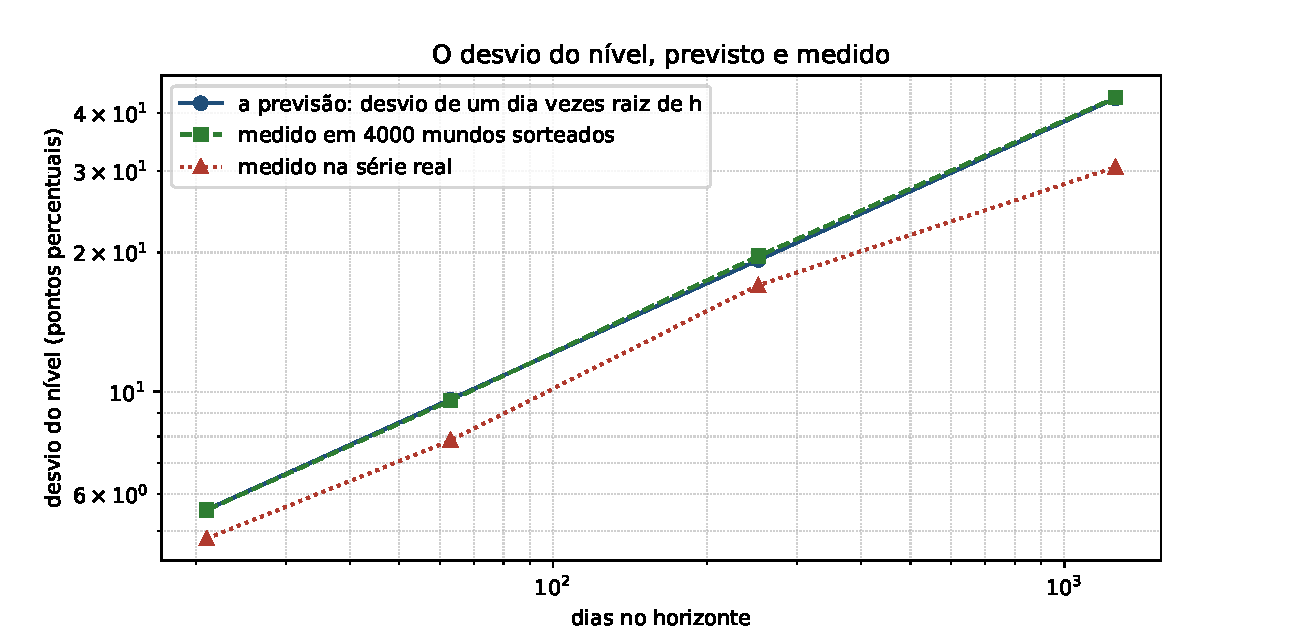
\includegraphics[width=\linewidth]{figuras/E22_soma_2.pdf}
  \caption{O desvio do nível contra o horizonte, nas três leituras. Os dois eixos estão em
    escala logarítmica, de modo que uma raiz aparece como reta de inclinação meio; a previsão e
    os mundos sorteados caem juntos, e a série real fica abaixo dos dois.}
  \label{fig:passo}
\end{figure}

A causa não está no tamanho dos dias: está na \textbf{ordem} deles. A autocorrelação de um dia nesta série vale
\numSomaRhoUm{} --- o dia de hoje tende a desfazer parte do que o de ontem andou ---, e a
previsão da raiz supõe justamente o contrário, dias independentes. Baralhando os retornos, de
modo que os mesmos dias enormes continuem todos lá e só a ordem morra, a razão no horizonte de um
mês vai a \numSomaBaralhadaRazaoVinteUm{} em \numSomaBaralhadaSorteios{} baralhamentos, contra
\numSomaRealVinteUmRazao{} do dado. Em cinco anos ela vai a
\numSomaBaralhadaRazaoMilDuzentosESessenta{}, e o que resta do buraco é do próprio estimador, que
mede janelas sobrepostas: a razão do horizonte longo é a de menor potência, e é a que menos
separa.

\begin{figure}[htbp]
  \centering
  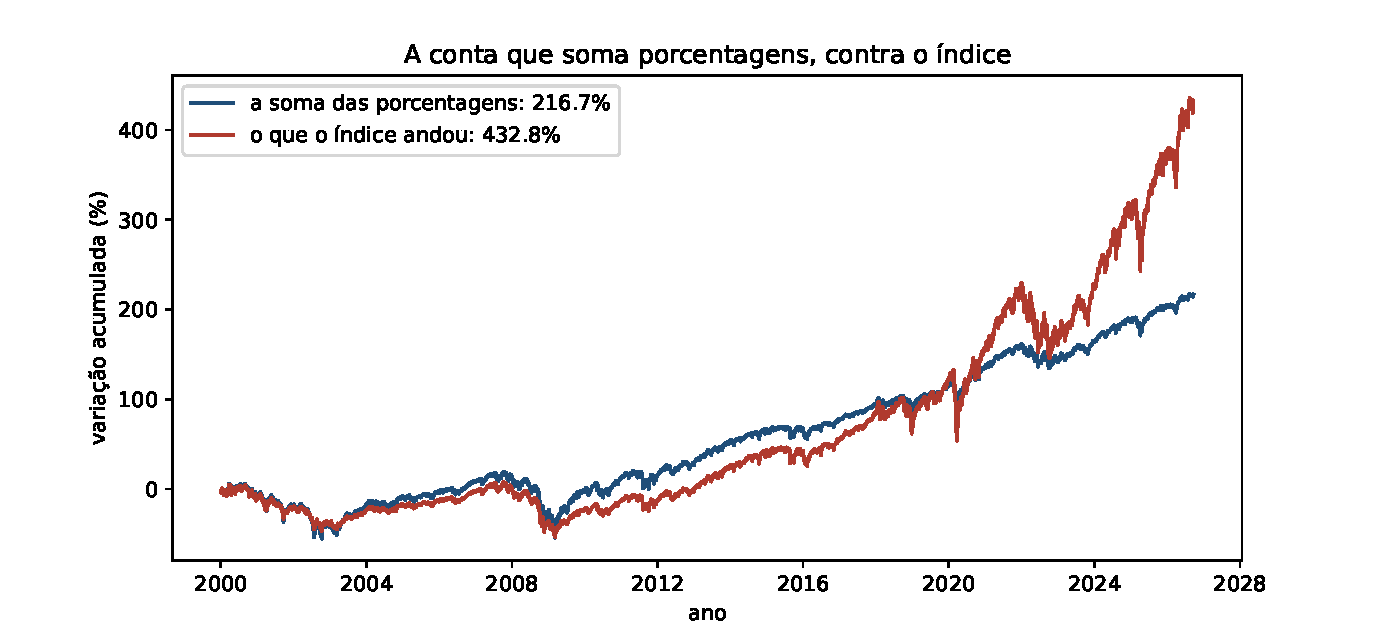
\includegraphics[width=\linewidth]{figuras/E22_soma_1.pdf}
  \caption{As duas somas, dia a dia, ao longo dos \numSomaSerieDias{} pregões. As curvas
    caminham juntas por anos, com a soma das porcentagens acima na maior parte do tempo, e se
    separam de vez no fim: o índice termina com mais que o dobro do que a soma entrega.}
  \label{fig:somas}
\end{figure}

O desenho mostra o mesmo que a conta: as duas curvas andam próximas por anos, e a distância
entre elas cresce com o tempo. Ela é pequena enquanto o nível anda pouco, e cresce com o
próprio nível --- que é o que uma multiplicação faz.

\section{A inclinação da banda em toda escala}

A seção anterior respondeu "quanto a banda da série fica abaixo da previsão" com um número
por horizonte --- e os quatro números dizem coisas diferentes, sem escada nenhuma entre eles.
Quem quer um número que valha para a série inteira tem a pergunta certa e o instrumento
errado: a razão num horizonte é uma leitura pontual, e a curva de \cref{fig:passo} tem
inclinação própria, esperando quem a meça.

% aterramento: atraso
% aterramento: passo-do-caminho
O instrumento mede o caminho em toda escala de uma vez. O \textbf{atraso} é o horizonte
entre os dois dias que entram na leitura: um dia, um mês de pregões, dois anos. O
\textbf{passo médio do caminho} é quanto o nível andou entre esses dois dias, em média ---
para cada atraso $h$, a média de $|\log p_{t+h} - \log p_t|$ sobre todas as janelas da
série, sobrepostas e sem dividir pelo atraso, o que é declaração: o que interessa é quanto o
passo cresce quando o atraso cresce. O exemplo mínimo cabe numa frase: no passeio puro,
quadruplicar o atraso dobra o passo médio.

A \cref{prop:passo} já contém essa frase. O passo típico de um passeio cresce com a raiz do
atraso, $\sigma\sqrt{h}$, de modo que contra o atraso em escala logarítmica o passo do
passeio é uma reta --- de inclinação um meio.

% aterramento: gama
A inclinação da reta é o objeto novo: o \textbf{expoente do caminho}, $\gamma$, um número
por série. E a leitura de Higuchi \cite{higuchi1988approach} é a de que essa inclinação é
um número repetível, que caracteriza a série que o produziu --- dita do outro lado, como
% aterramento: dimensao-do-caminho
dimensão: a \textbf{dimensão do caminho} é $2 - \gamma$. No sorteio puro a inclinação é meio
e a dimensão, três meios; caminhos mais lisos aproximam um, e caminhos que enchem a página
chegam a dois.

A medição corre nos três lugares de sempre: \numExpoenteMundos{} mundos do passeio puro, a
série, e os \numExpoenteSorteios{} baralhamentos da seção anterior --- o mesmo estimador,
os mesmos \numExpoenteAtrasos{} atrasos, de um dia a \numExpoenteAtrasoMaximo{} pregões, e
todo atraso com menos de \numExpoenteJanelasMinimas{} janelas de sobra fica de fora do
ajuste.

Nos mundos, a inclinação medida é \numExpoenteGammaPasseio{}, com dispersão
\numExpoenteGammaPasseioDispersao{} entre mundos --- meio, e a dimensão
\numExpoenteDimensaoPasseio{}, três meios. A régua da \cref{prop:passo}, agora como número
medido: \cref{fig:escala} mostra a régua caindo junto com o meio dos mundos.

Na série, o número é \numExpoenteGammaReal{} --- e a régua de ordem diz o que ele é. O
mesmo estimador nos baralhamentos dá \numExpoenteGammaBaralhadoMedia{}, com dispersão
\numExpoenteGammaBaralhadoDispersao{}: colado no da série, e as dimensões vêm coladas
junto, \numExpoenteDimensaoReal{} contra \numExpoenteDimensaoBaralhadoMedia{}. A inclinação global é carregada pelos tamanhos dos dias --- baralhar a ordem deixa o
número onde está. E a compressão que a
seção anterior mediu, a banda da série abaixo da prevista, mora na forma da curva, de um
jeito que o número global não vê --- a série nasce junto do baralhamento no atraso de um dia
(os mesmos dias), corre abaixo do meio dos mundos nos atrasos curtos e médios e a
alcança no maior deles; o baralhado, que também começa abaixo do meio dos mundos, o ultrapassa
na faixa curta. A \cref{fig:gamas} mostra o mesmo na contagem: as inclinações dos mundos se
acumulam no meio, as do baralhado um pouco à direita, e a linha da série cai dentro da
pilha do baralhado.

A forma aparece quando a inclinação é lida por faixa de atraso:

\begin{table}[htbp]
  \centering
  \small
  \resizebox{\linewidth}{!}{%
  \begin{tabular}{lrrr}
    \hline
    atrasos da faixa & a série & os mundos & o baralhado \\
    \hline
    um a oito dias & \numExpoenteGammaFaixaCurtaReal & \numExpoenteGammaFaixaCurtaPasseio & \numExpoenteGammaFaixaCurtaBaralhado \\
    dezesseis a sessenta e quatro & \numExpoenteGammaFaixaMediaReal & \numExpoenteGammaFaixaMediaPasseio & \numExpoenteGammaFaixaMediaBaralhado \\
    cento e vinte e oito a quinhentos e doze & \numExpoenteGammaFaixaLongaReal & \numExpoenteGammaFaixaLongaPasseio & \numExpoenteGammaFaixaLongaBaralhado \\
    \hline
  \end{tabular}}
  \caption{O expoente do caminho lido por faixa de atraso. Nos mundos, meio em toda faixa;
    na série, a inclinação anda com a escala; no baralhado, bem mais parada.}
  \label{tab:faixas}
\end{table}

Nos mundos a inclinação é meio em toda faixa --- a régua não depende da escala. Na série
ela anda: o dia que desfaz parte do dia anterior (\numSomaRhoUm{}) achata a faixa curta,
\numExpoenteGammaFaixaCurtaReal{} contra \numExpoenteGammaFaixaCurtaBaralhado{} do
baralhado --- a ordem, que o número global não via, aparece aqui ---, e na faixa longa a
série passa o próprio baralhado, \numExpoenteGammaFaixaLongaReal{} contra
\numExpoenteGammaFaixaLongaBaralhado. Entre os extremos, a inclinação sobe de
\numExpoenteGammaFaixaCurtaReal{} a \numExpoenteGammaFaixaLongaReal.

O que a inclinação entregou, e o que ela cobrou. Entregou: a régua de meio virou número
medido, a série ganhou o seu, e a régua de ordem disse do que o número é feito --- os
tamanhos dos dias. Cobrou: um número só descreve a série se a escala vier junto, e a ordem
dos dias, que decide a banda do mês, só aparece lendo faixa por faixa. O número que
caracteriza a série existe e é repetível; descrever a série com ele é outra história.

\begin{figure}[htbp]
  \centering
  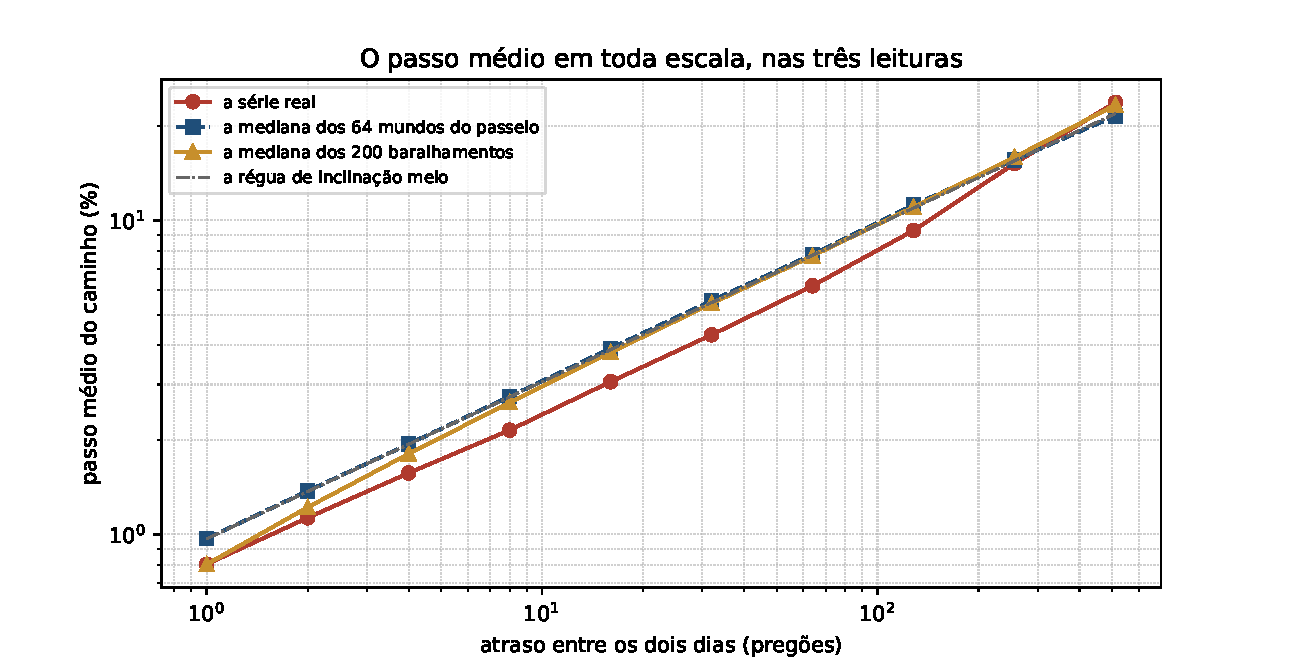
\includegraphics[width=\textwidth]{figuras/E44_expoente_1.pdf}
  \caption{O passo médio do caminho contra o atraso, nos dois eixos em escala logarítmica.
    A série nasce junto do baralhamento no atraso de um dia --- os mesmos dias ---, corre
    abaixo do meio dos mundos nos atrasos curtos e médios e a alcança no maior deles; o
    baralhado começa abaixo do meio dos mundos e o ultrapassa dentro da faixa curta; a régua de
    meio cai junto com o meio dos mundos.}
  \label{fig:escala}
\end{figure}

\begin{figure}[htbp]
  \centering
  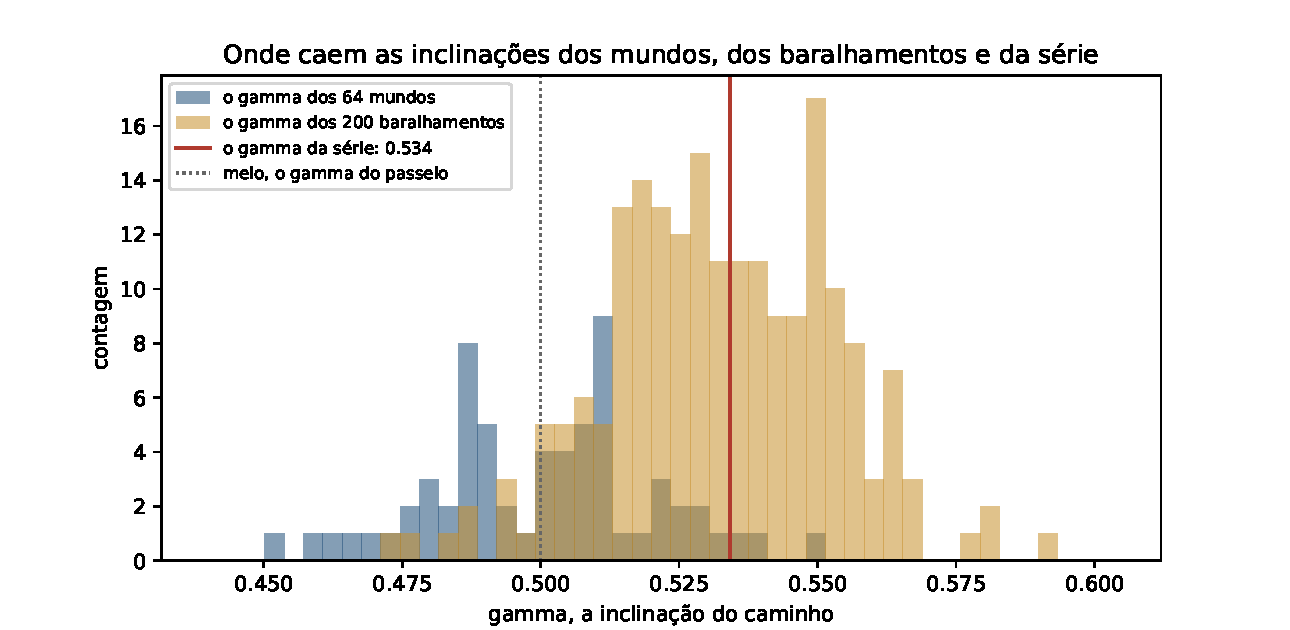
\includegraphics[width=\textwidth]{figuras/E44_expoente_2.pdf}
  \caption{A inclinação de cada mundo e de cada baralhamento, com a da série marcada. As
    pilhas se acumulam perto de meio --- a dos mundos em cima dele, a do baralhado um pouco
    à direita --- e a linha da série cai dentro da pilha do baralhamento: o expoente global
    é um número dos tamanhos dos dias.}
  \label{fig:gamas}
\end{figure}

\section{O que fica}

Ficam os dois objetos que o resto do livro usa sem dizer: o \textbf{nível}, que é o preço, e o
\textbf{incremento}, que é o que o dia acrescentou. Fica a ponte entre eles, e ela é o
logaritmo: somar retornos é o mesmo que olhar a razão entre dois preços, exatamente. E fica a
banda do nível, que cresce com a raiz do horizonte --- medida em \numSomaMundos{} mundos, e
posta contra o dado real, onde ela exagera porque o dia de hoje desfaz parte do que o de
ontem andou.

A pergunta da noite continua de pé, e agora se vê o tamanho dela. A banda do nível se alarga
com o horizonte, e o que se quer saber é quanto se pode perder amanhã: uma resposta que não
pode ser uma linha fixa, porque a linha não se alarga. Medir o dia ruim exige erguer uma linha
sobre os piores dias do passado e olhar o que ficou abaixo dela --- e é essa linha que o
capítulo seguinte constrói.
